\qquad O \textit{Q\&A system} desenvolvido suporta várias funcionalidades que consideramos essenciais. O nosso objetivo era a criação de um sistema eficiente e intuitivo. Neste sentido, delineamos um conjunto de metas a atingir ao longo da realização do projeto, nomeadamente, funcionalidades a serem suportadas pelo sistema a nível da sua capacidade de resposta.

A lista é a que se segue:
\begin{itemize}
    \item \textit{Case} das letras (maiúsculo/minúsculo) não interferir com o reconhecimento da pergunta;
    \item Reconhecer perguntas que terminem em vários/múltiplos sinais de pontuação;
    \item Devolver a resposta guardada na Base de Conhecimento cuja intenção seja o mais semelhante à questão colocada;
    \item Caso não haja uma correspondência que se destaque de entre as existentes, havendo várias com o mesmo nível de igualdade, devolver essas mesmas respostas;
    \item Informar o utilizador da ausência de informação relativa à questão colocada;
    \item Reconhecer várias perguntas numa só questão.
\end{itemize}

Estes objetivos foram alcançados, sendo possível verificar na figura \ref{fig:funcs} \textit{inputs} sintaticamente corretos, isto é, que o sistema reconhece conforme as regras definidas.  

\begin{figure}[H]
\begin{center}
    \fbox{
    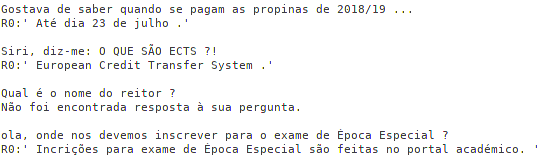
\includegraphics[width = 0.9\textwidth, keepaspectratio]{imagens/ex_funcs.png}
    }
    \caption{Exemplo do funcionamento do \textit{Q\&A System FAQ UMinho}}
    \label{fig:funcs}
\end{center}
\end{figure}




